\subsection{Capillary Viscometer} \label{sec:aufgabe3}
For the strength of the flow, we use:
\begin{equation}
i = \frac{V}{t}
\end{equation}
The pressure of the water can be calculated with:
\begin{equation}
p = \rho \cdot h \cdot g
\end{equation}
where $V$ is the Volume and $t$ the time.\\
The density of water is $\rho = \unit[997.6]{kg/m^3}$ at a temperature of $T = 22.9 \C$.%
\footnote{\url{https://www.wolframalpha.com/input/?i=density+of+water+at+22.9+celsius}}\\
For the height, we assume an error of $\unit[4]{mm}$ because the level of the water was hard to see through the plastic. The error of the time should be about $\unit[1]{s}$, the temperature error is at $\unit[0.2]{\C}$, which leads to an error of the density with $\Delta \rho = \pm \unit[0.1]{kg/m^3}$. The error of the mass is approximately $\unit[0.002]{g}$ (measuring the empty cylinder before and after the experiment). $\Delta p$ is therefore equal to $\unit[0.041]{kPa}$ (at the max. height).
The error for the strength of the flow adds up to $\unit[1.74\e{-3}]{cm^3/s}$.\\As the task formulation tells us, there are some more sources of errors, e.\,g. physical effects, which will be included in the linear regression.

\begin{figure}
\begin{center}
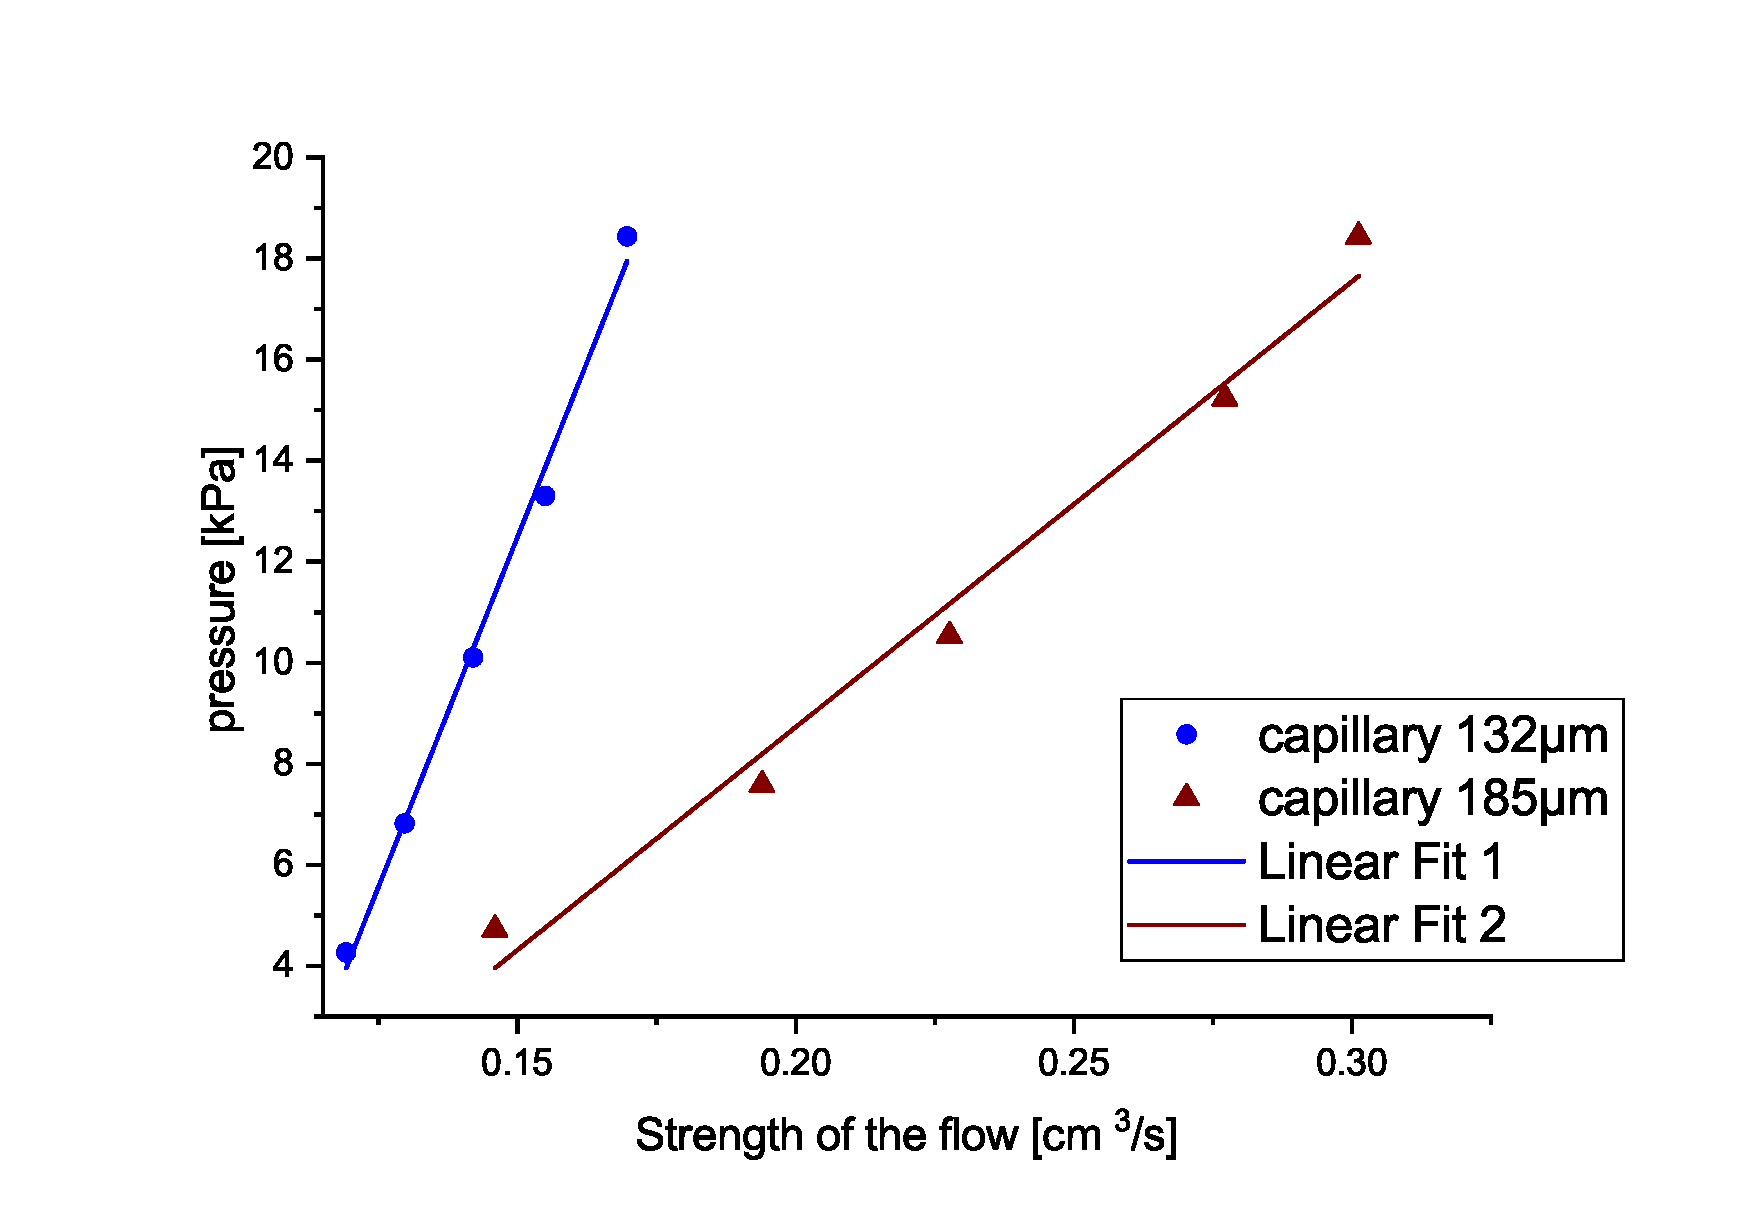
\includegraphics[width=0.7\textwidth]{Bilder/aufgabe2.eps}
\caption{Measuring $\Delta i$ for two different capillary radii}
\label{fig:aufgabe2}
\end{center}
\end{figure}

The graph of the measured values is shown in figure \ref{fig:aufgabe2}. With linear regression we get the following values and errors:
\begin{align*}
W_1 &= \unit[(276.95 \pm 11.87)]{\frac{kPa s}{cm^3}}\\
W_2 &= \unit[(88.18 \pm 6.64)]{\frac{kPa s}{cm^3}}
\end{align*}
The length of the first capillary is $l_1 = \unit[(29.5 \pm 0.025)]{cm}$ and $l_2 = \unit[(3.52 \pm 0.025)]{cm}$
With the help of formula \ref{eq:pressure} it is possible to calculate the viscosity $\eta$. The errors are -- as always -- calculated with the derivatives (like shown in section \ref{sec:aufgabe2}).
\begin{align*}
\eta_1 &= \unit[(1.12 \pm 0.22)]{mPa s}   \\
\eta_2 &= \unit[(1.15 \pm 0.28)]{mPa s}
\end{align*}
Considering the error, the values lie withing values found in literature (see section \ref{sec:aufgabe1}).




